%
% resources.tex
%
% Copyright (C) 2018 by Andre Martins Pio de Mattos <andrempmattos@gmail.com>.
%
% Internship Report
%
% This work is licensed under the Creative Commons Attribution-ShareAlike 4.0
% International License. To view a copy of this license,
% visit http://creativecommons.org/licenses/by-sa/4.0/.
%

%
% \brief Title page.
%
% \author Andre Martins Pio de Mattos <andrempmattos@gmail.com>
%
% \version 0.1.0
%
% \date 08/09/2019
%

\newpage

%================================================================================

\section{Development} \label{sec:development}

The following topics will cover the entire payload development process in details, focusing on the architecture, methods, and technologies, besides the actual development steps and results. Some organizational and work activities aspects are shortly mentioned or placed as annexes, unless essential for the comprehension of the measures and approaches adopted throughout the development, since the focus of this work is the technological challenges and analysis, and the architectural proposals. The \autoref{fig:payload_demo} presents the final version (Flight Model) of the developed payload. 

\begin{figure}[!ht]
    \begin{center}
        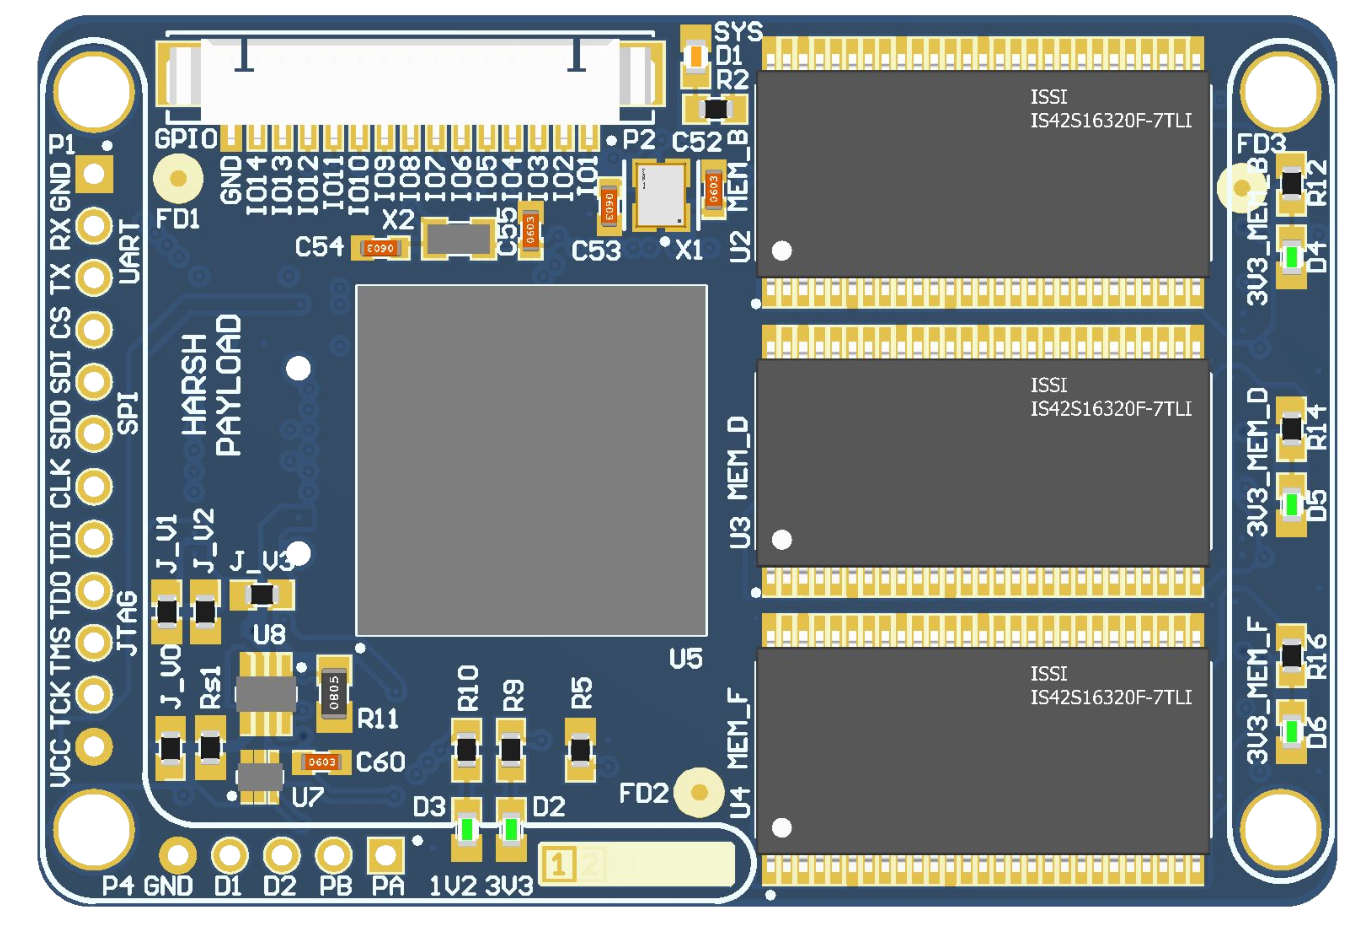
\includegraphics[width=0.7\textwidth]{figures/harsh_pcb_top.png}
        \caption{Preview of the developed payload.}
        \label{fig:payload_demo}
    \end{center}
\end{figure}

%================================================================================

\subsection{System Overview}

In order to accomplish the payload requirements, the development process reached different stages of completion: prototype phase, engineering model and flight model. These categories are a simplification of the system engineering phases definition, which generally define a deliverable and a associated review. For this reason, an overview of each stage of the system is provided to ease the understanding of the project evolution and an iterative architectural conception. The \autoref{tab:summary_phases} summarizes the delivered features in each phase and overall standards compliance.

\begin{table}[!h]
    \begin{center}
        \begin{tabular}{ l|ccc }
            \toprule
            \textit{Features and standards} & \textit{Prototype} & \textit{Engineering Model} & \textit{Flight Model} \\
            \midrule
            System control and management   & x & x & x \\
            Reliable radiation controller   & x & x & x \\
            Radiation hardened board        &   & x & x \\
            Single SDRAM memory access      & x & x & x \\
            Multiple SDRAM memory access    &   & x & x \\
            Static memory test algorithms   &   & x & x \\
            Dynamic memory test algorithms  &   &   & x \\
            Frequency test algorithms       &   &   & x \\
            Refresh rate test algorithms    &   &   & x \\
            UART communication interface    & x & x & x \\
            SPI communication interface     &   & x & x \\
            I2C communication interface     &   &   &   \\
            CAN communication interface     &   &   &   \\
            Watchdog timer protection       &   & x & x \\
            Low power mode operation        &   & x & x \\
            FSP protocol implemented        &   & x & x \\
            Debug logging routines          & x & x & x \\
            Experiment routines             &   & x & x \\
            Communication routines          &   & x & x \\
            System housekeeping routines    &   & x & x \\
            Reliable FreeRTOS instance      &   & x & x \\
            Firmware reliability review     &   & x & x \\
            Hardware reliability review     &   &   & x \\
            \bottomrule
        \end{tabular}
    \end{center}
    \caption{Project phase progress according to the specifications.}
    \label{tab:summary_phases}
\end{table}

%--------------------------------------------------------------------------------

\subsubsection{Prototype}

During the prototype phase, the base architecture and components of the design were selected to fulfill the payload requirements. The SDRAM memories controller was the first aspect to be defined due to its importance inside the payload. This definition lead for a FPGA architecture, which could provide the necessary design flexibility and port connections, high frequencies support, and parallel execution during memory operations. Then, among different technologies and vendor options, the SmartFusion2 family from Microsemi emerged as a good trade-off between performance, power consumption, and reliability. Also, these devices have an embedded ARM Cortex-M3 processor, several useful on-chip peripherals and the advantage of being flash based, which provide a radiation hardened attribute.

Then, in order to test and validate the first design concepts, the next stage was selecting a suitable development board. Among the different options provided for this device family, the SMF2000 development kit were the best solution for the prototype conception. This board standout due to its low price, simple architecture, and all the necessary features, including a SDR SDRAM memory for the first design validations. The \autoref{fig:smf_2000} presents the board and its components highlighted: in yellow, the FTDI used to format the FPGA bitstream, debug and send log messages; in orange, the 64Mb (or 8MB) SDR SDRAM; and in red, the M2S010 SoC FPGA chip.

\begin{figure}[!ht]
    \begin{center}
        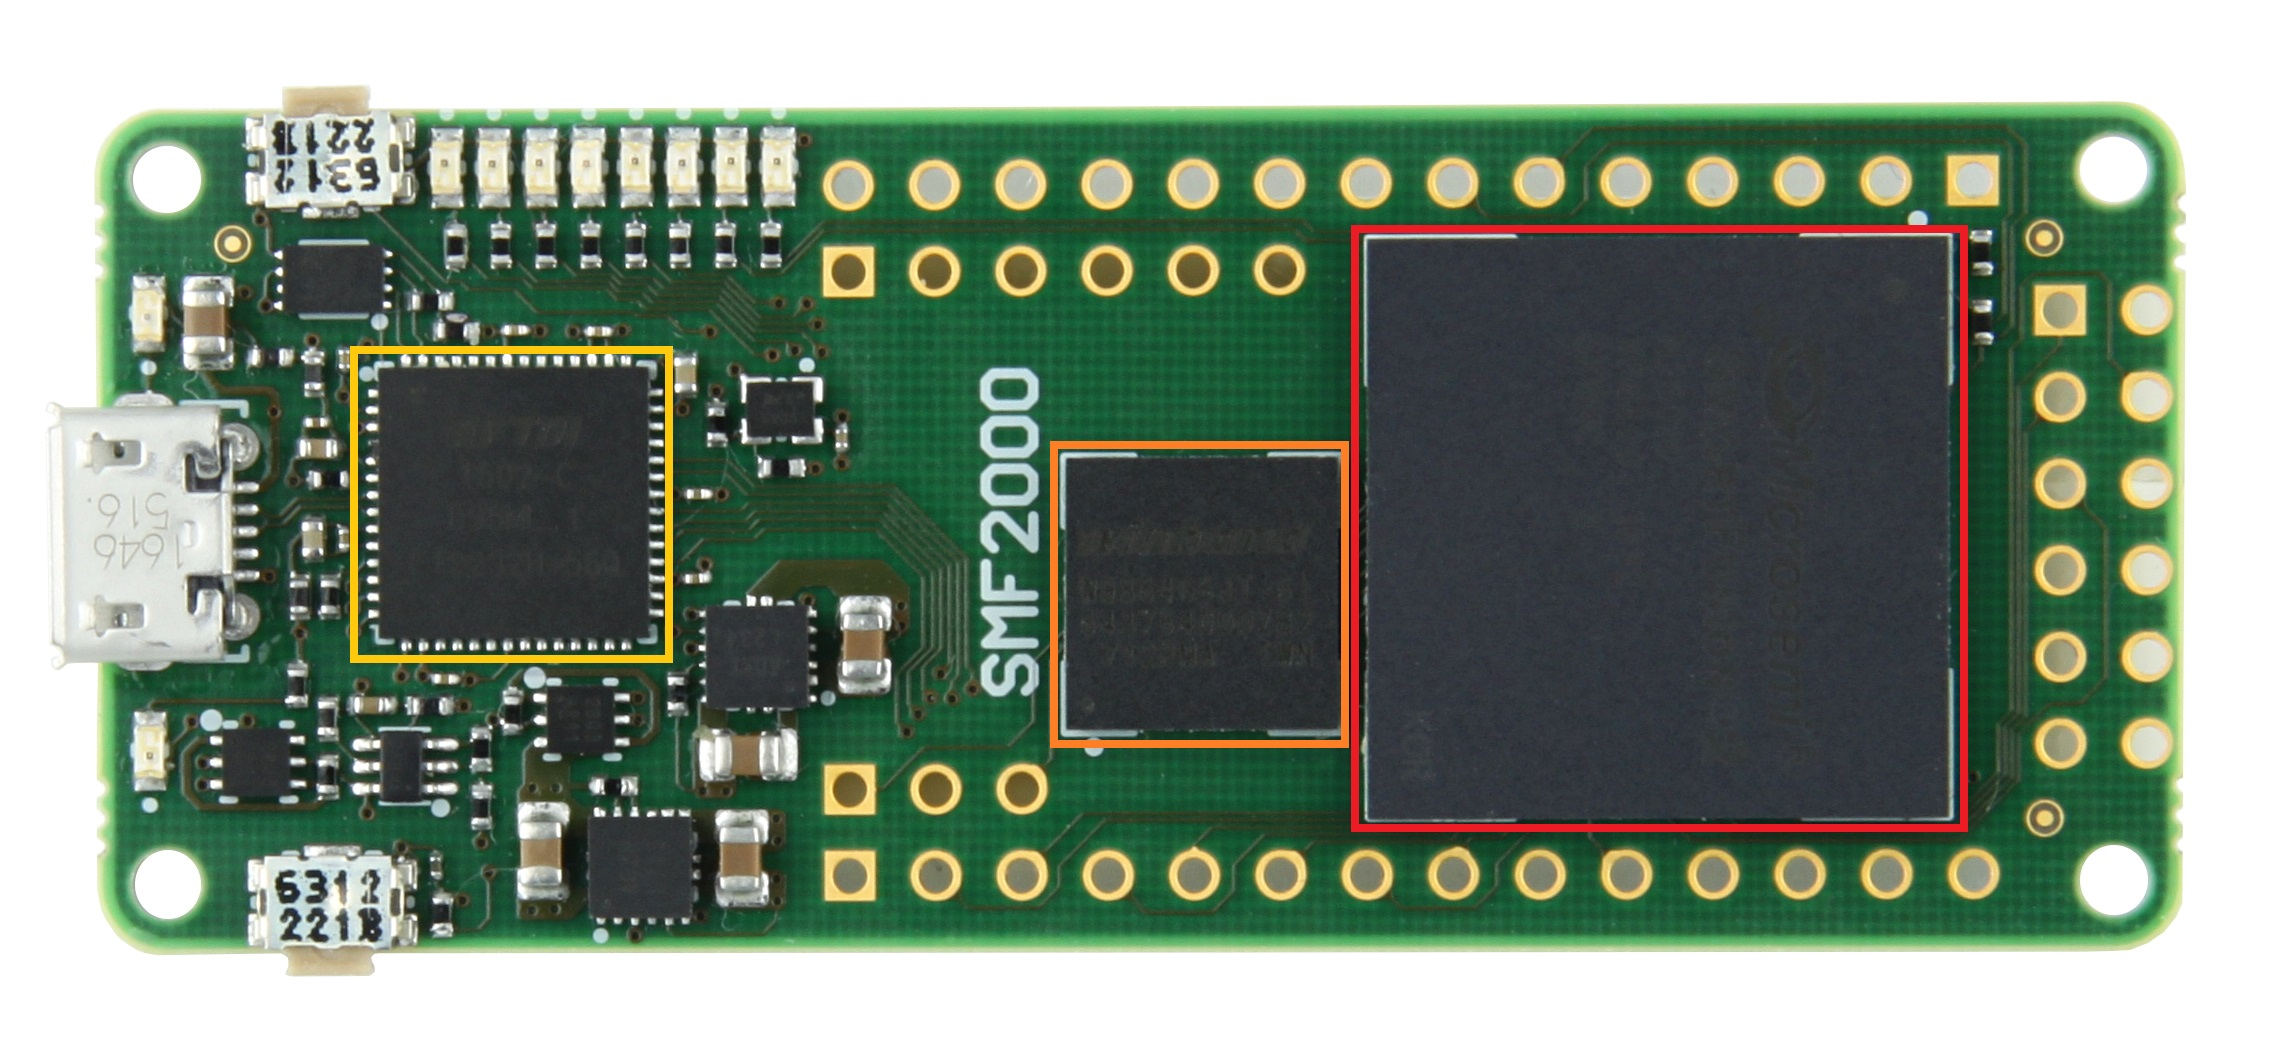
\includegraphics[width=0.75\textwidth]{figures/smf2000_top.jpg}
        \caption{Development board used during the prototype phase.}
        \label{fig:smf_2000}
    \end{center}
\end{figure}

Regarding the delivered features of the prototype, shown in the \autoref{tab:summary_phases}, the base SoC design solution and the minimal system firmware were developed to attend the most critical aspects of payload, which includes the memories control and tests, simple communication routines, and usage of the internal non-volatile memory to store the firmware sources. Since the FPGA is flash based, a non-volatile memory, the bitstream is retained indefinitely and any formatting routine is necessary after system resets. 

%--------------------------------------------------------------------------------

\subsubsection{Engineering Model}

After the prototyping phase, the engineering model started to be developed, considering the previous phase review outputs. Since the first approach was using a development kit, the major external revisions focus on the FPGA SoC architecture and the software definitions. Then, the first iteration of hardware development was based on the SMF2000 and to reduce further changes, this version intended to be as close as possible of the flight model. Interfaces, connectors and the memories were the major changes from the development kit, besides the FPGA assignments and the board shape itself. The \autoref{fig:hardware_architecture_simplified} presents a simplified architecture diagram of the engineering model, which includes the hardware and SoC FPGA modules.

\begin{figure}[!ht]
    \begin{center}
        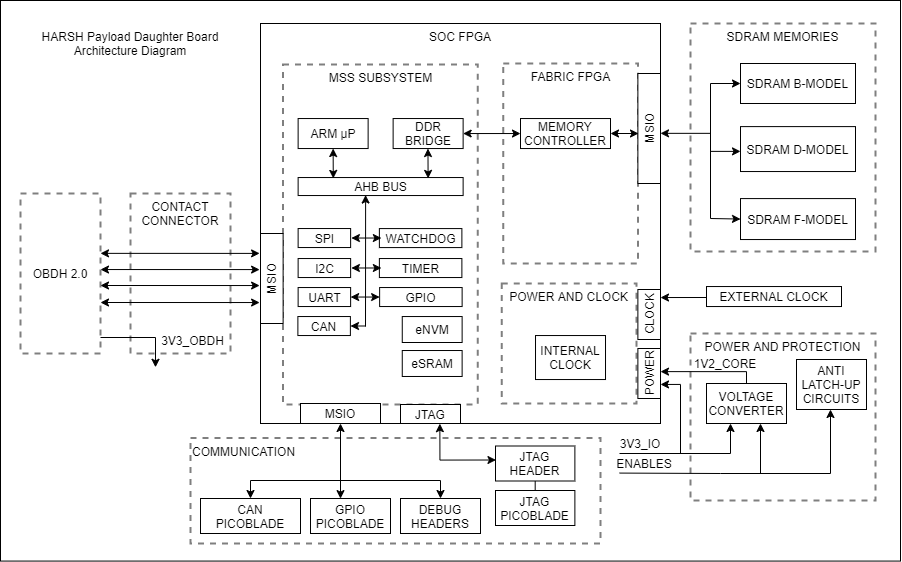
\includegraphics[width=0.95\textwidth]{figures/hardware_architecture_simplified.png}
        \caption{Simplified engineering model architecture.}
        \label{fig:hardware_architecture_simplified}
    \end{center}
\end{figure}

In order to visualize the integration with the GOLDS-UFSC OBDH, some conceptual assemblies were performed during the development. The \autoref{fig:conceptual_model} presents one of these integration setups and provide a visual understanding of both modules, their mechanical connection and electrical interface through the contact connector.

\begin{figure}[!ht]
    \begin{center}
        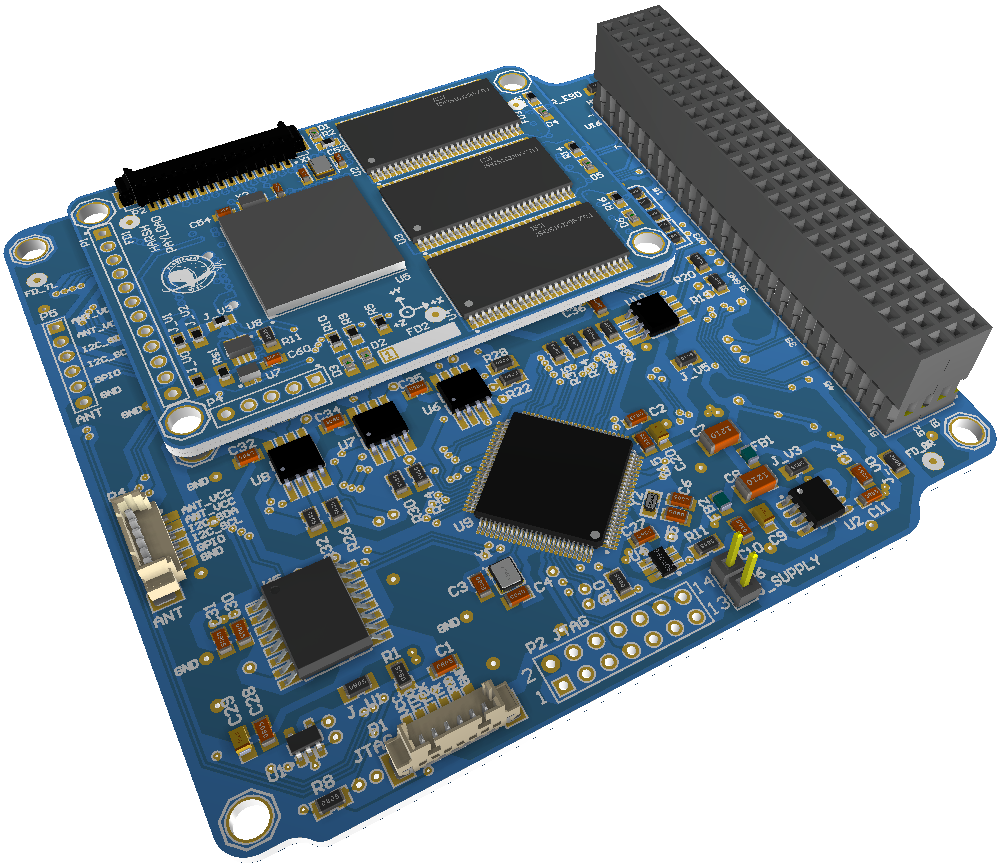
\includegraphics[width=0.65\textwidth]{figures/conceptual_model.png}
        \caption{Conceptual payload model integrated with GOLDS-UFSC OBDH.}
        \label{fig:conceptual_model}
    \end{center}
\end{figure}

In summary, the engineering model review revealed that the hardware design and the SoC FPGA solution are adequate to the payload mission and requirements as a flight version. The firmware, showing the basic operation and experiments, presented satisfactory overall stability, but it was decided to refactor some routines, perform more specific tests, and improve the reliability and redundancy of some modules.   

%--------------------------------------------------------------------------------

\subsubsection{Flight Model}

Regarding the flight qualified model, the major changes from the engineering version were the system firmware and the experiment algorithms. These modifications were important to improve the experiment execution and provide better results. Also, the integration tests revealed some weak points and non-reliable management routine implementations that might led to critical failures. Then, in order to solve these issues, the firmware was updated, tested and the design reviewed. These changes were related to the memory controller refresh rate, data acquisition and some synchronization issues. The design presented in this document covers the updated and functional implementation.

%================================================================================

\newpage

\subsection{SoC FPGA Architecture} \label{subsec:fpga}

The payload core subsystem is the SoC FPGA, which provide the system control and management due to embedded microprocessor, memory controller, communication interfaces and main peripherals. The device settles the main functionalities of the payload system, then using a radiation hardened technology improves the overall system reliability and permits the analysis of the memory faults within the absence of controller errors. Also, the SmartFusion2 family is suitable for critical applications due to its intrinsic robustness, high density die, high-performance and availability of a wide variety of peripherals
features. Moreover, these devices has a historic of utilization in space applications and demonstrates satisfactory overall performance and reliability. The \autoref{fig:die} provide a internal physical architecture overview of the SmartFusion2 devices. The following sections describe the SoC system implemented in the M2S010 FPGA, part of this device family, and include its simulation and test results.

\begin{figure}[!ht]
    \begin{center}
        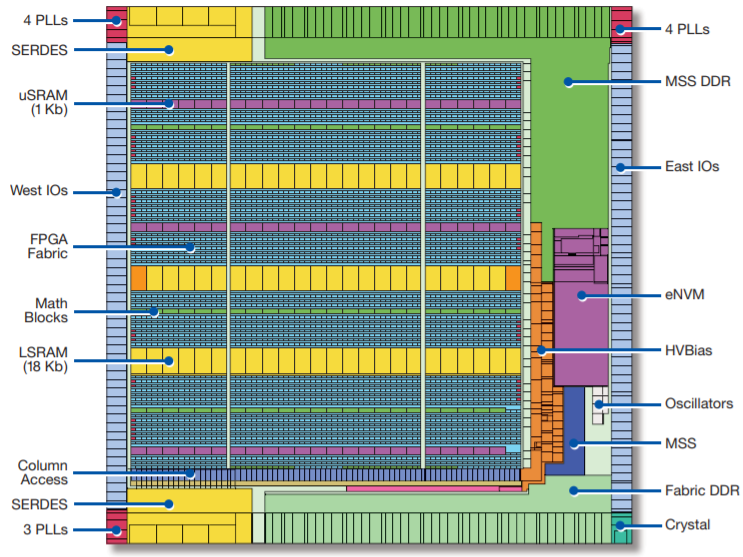
\includegraphics[width=0.8\textwidth]{figures/die.png}
        \caption{FPGA die overview.}
        \label{fig:die}
    \end{center}
\end{figure}

%--------------------------------------------------------------------------------

\subsubsection{Design Overview}

The SoC architecture embedded in the FPGA chip has several features and allows each subsystem to be enabled or disabled in the design, in order to reduce the power consumption. The device is subdivided in two different parts: the Microcontroller Subsystem (MSS), with a fixed implementation, and the FPGA Fabric, where the user modules and configurations are implemented. For this project, both parts are employed to create the payload required capabilities and define the core design: controller, using the ARM Cortex-M3 processor; Soft Memory Controller(SMC) for the SDRAM management, in the FPGA Fabric section; serial communication (MMUART\textunderscore0), SPI\textunderscore0, I2C\textunderscore0); Watchdog timer, for system protection; RTC and timers, for synchronization; GPIO ports; Embedded Non-Volatile Memory (eNVM\textunderscore0) for code sources storage; and debug, using the System Controller for JTAG interface. The following topics details each subsystem characteristics and operation. Also, the \autoref{fig:feature_overview} presents a simplified diagram of the built-in internal available modules.

\begin{figure}[!ht]
    \begin{center}
        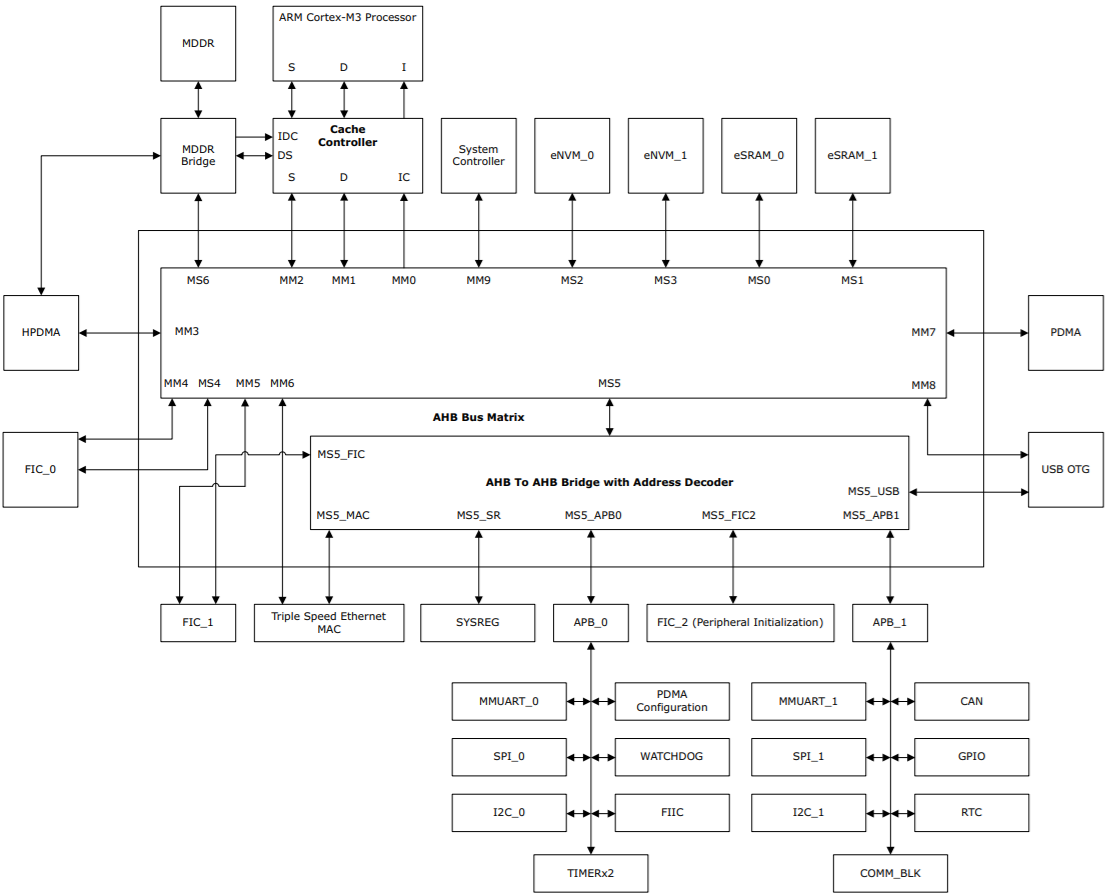
\includegraphics[width=\textwidth]{figures/feature_overview.png}
        \caption{Internal architecture diagram overview.}
        \label{fig:feature_overview}
    \end{center}
\end{figure}

\paragraph{Microprocessor} \mbox{}\\

In the SoC architecture, the processing unit is a hard core instance of an ARM Cortex-M3 microprocessor. The unit has a low power consumption design and intend to accomplish the deeply embedded applications requirements. This processor consists in a 32-bit RISC architecture with 3-stage pipeline that provide enough processing performance for the payload routines and algorithms. In order to provide the utility features for this device, the SoC design includes a set of peripherals, which combine communication, timers, system memories, watchdog and debug modules. When disabled, these subsystems are hold in low power mode and provide customization during the development that contribute for the feasibility in power constrained applications. Also, the system uses the ARM Advanced Microcontroller Bus Architecture (AMBA) as interface for the peripherals and the FPGA fabric devices, employing the Advanced High-performance Bus (AHB) protocol in the communications.

\paragraph{Memory Controller} \mbox{}\\

In order to manage the SDRAM memories, a controller instantiated in the FPGA fabric is used for the external interface with these devices. In this architecture, the controller is shared among the memories since the operations campaigns are performed separately for each device and concerning timing the memories are compatible. Moreover, due to the similar internal logical architectures, despite the manufacturing differences, the memories are similar in operation and constraints. \autoref{fig:hpdma} describes the interfaces used for the controller from the processor until the external interface. The processor, a master in the AHB bus, requests data operations for the DDR Bridge that redirect these commands for the memory controller, using a AHB to AXI interface. Then, the controller, besides the regular management operations, handles the communication and control signals through the MSIO ports to the actual memory. Since the SDRAM chips are connected in parallel in the same MSIO ports, the controller uses chip select signals to enable the correct device.  

\begin{figure}[!ht]
    \begin{center}
        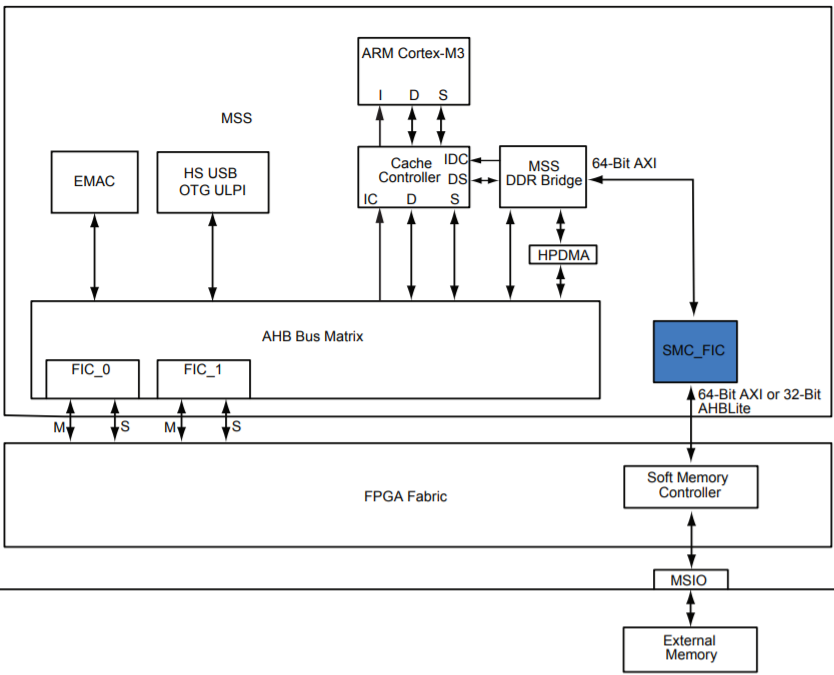
\includegraphics[width=0.7\textwidth]{figures/hpdma.png}
        \caption{Memory controller interfaces overview.}
        \label{fig:hpdma}
    \end{center}
\end{figure}

This controller is part of the catalog collection provided by the SoC FPGA vendor, which provides several ported IP Cores for the fabric implementation. The used core is designed for SDR SDRAM memories and adapted to be connected to an Advanced eXtensible Interface (AXI). The \autoref{fig:core_sdr_axi} shows a simplified diagram of this IP core. In summary, this module receive operation requests through the AXI bus and the internal controller handles this demands, generating the formatted operation frame for the actual memory controller and handling its responses for the requester. However, since the MSS subsystem (the requester) architecture provide an AHB interface, a converter is required to properly handle the protocol exchange for an AXI bus. Also, this module is provided in the vendor catalog and do not require external control, besides the reset signal.

\begin{figure}[!ht]
    \begin{center}
        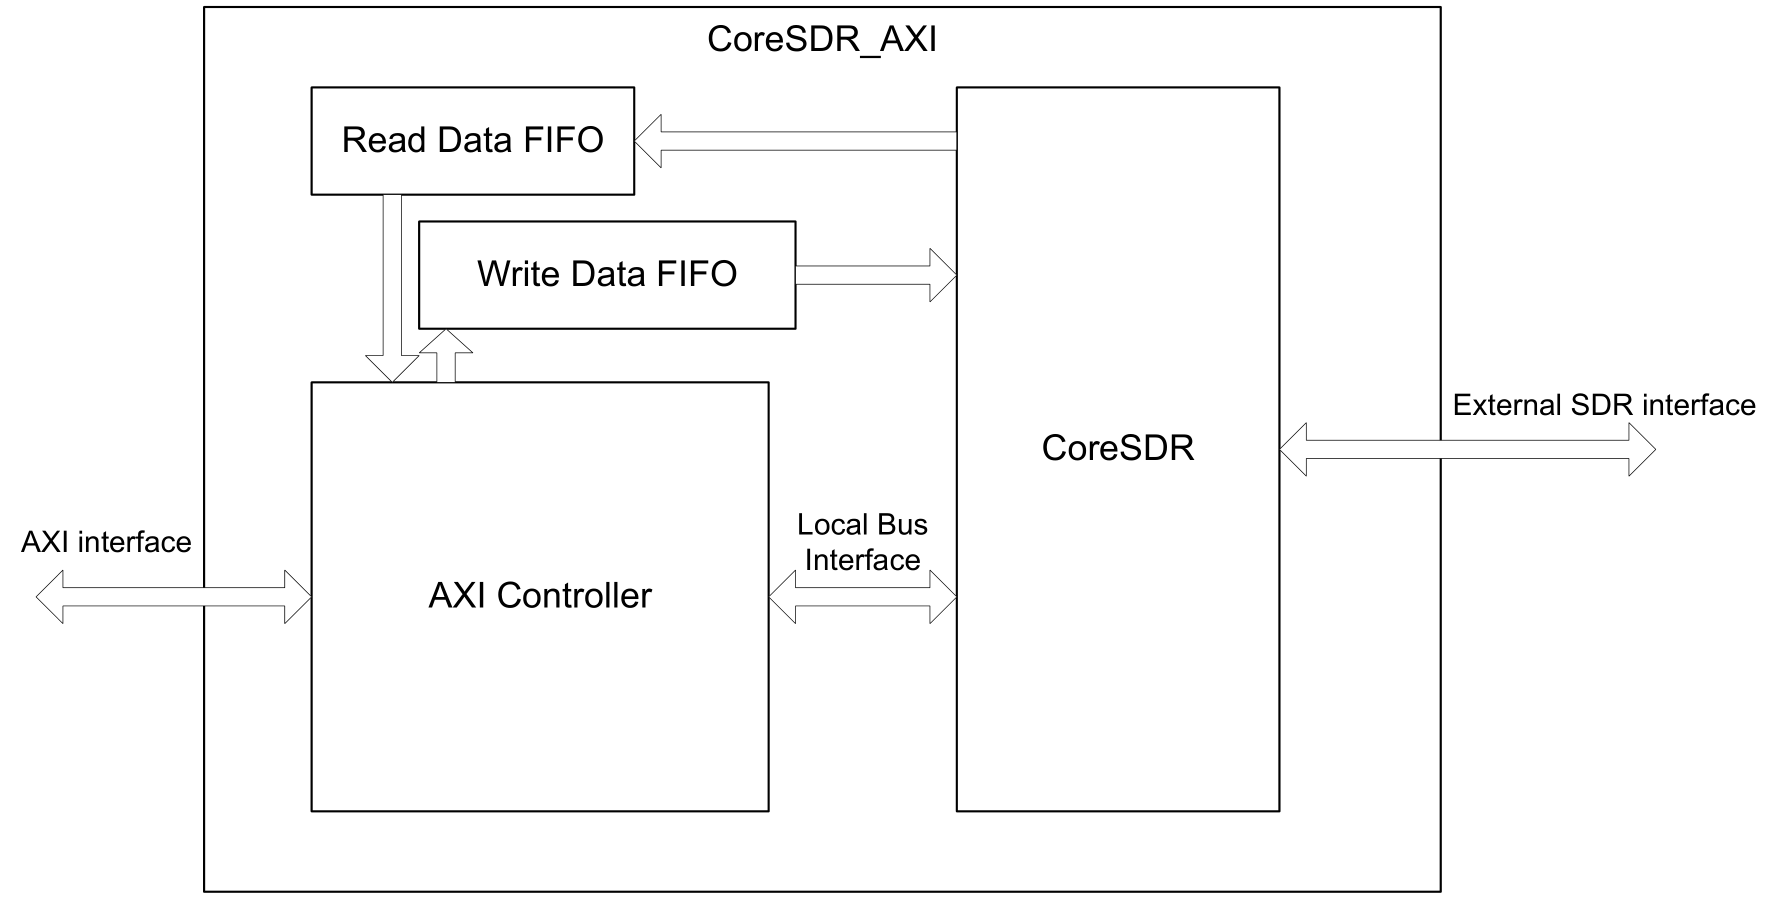
\includegraphics[width=0.85\textwidth]{figures/core_sdr_axi.png}
        \caption{Core SDR wrapped for an AXI interface architecture.}
        \label{fig:core_sdr_axi}
    \end{center}
\end{figure}

The CoreSDR is the controller that manage the memory communication, generating the control signal within the time constraints. It receives the operation requests, data length and addresses from the AXI controller and the data from the write buffer in case of a write operation. The input address is structure as described in the \autoref{fig:addr_scheme}. This scheme is important to determine which memory should be accessed in relation to the input address, where the three most significant bits are decoded in up to eight chip selects and the others bits to set the column, row and bank. When an encoded chip select bit changes, it means that the address space of that memory ends and the next starts. This scheme allows the usage of up to eight memories without the need of additional controllers or external interfaces. 

\begin{figure}[!ht]
    \begin{center}
        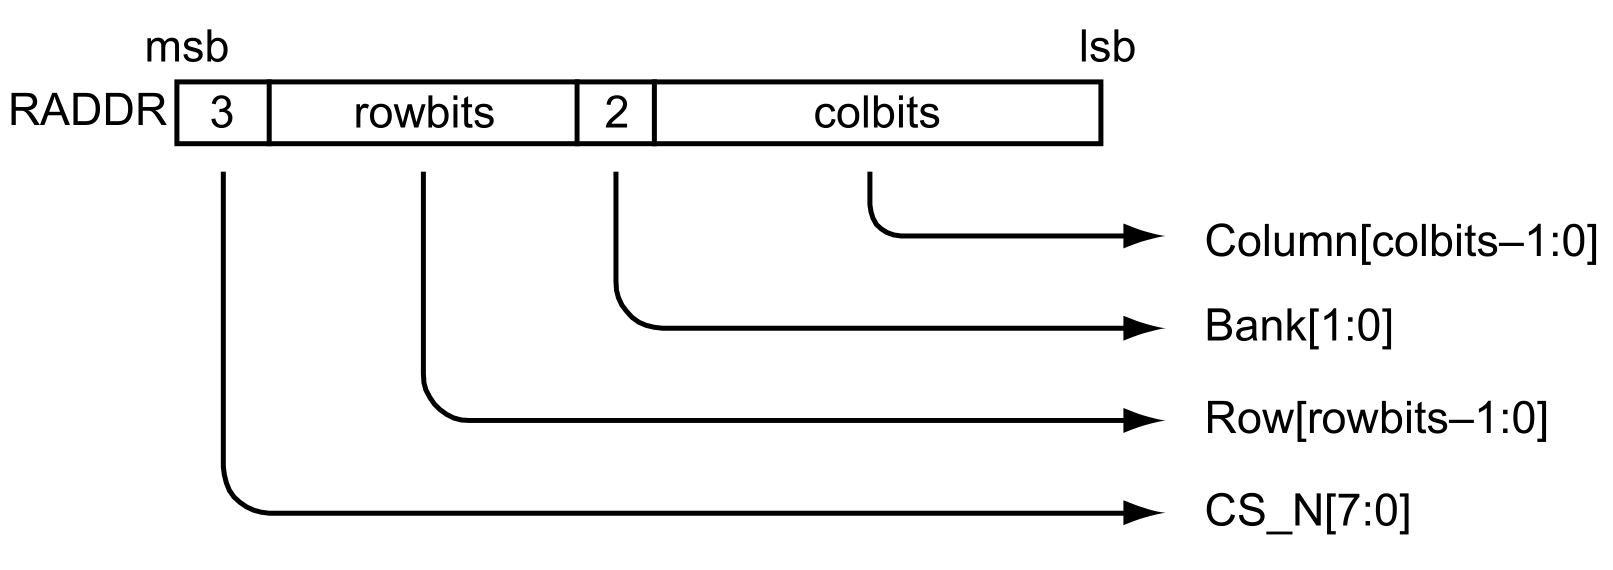
\includegraphics[width=0.6\textwidth]{figures/addr_scheme_core_sdr.png}
        \caption{Core SDR Address scheme overview.}
        \label{fig:addr_scheme}
    \end{center}
\end{figure}

The \autoref{fig:core_sdr} shows the internal modules of the controller and the corresponding signals. The output signals are directly connected to the SDRAM memories: RAS, CAS and WE determine the requested commands; SA and BA set the target addresses; DQM is a mask for bytes within a word; CKE is used to enable the clock in the memory; CS activate the selected memory; DQ is used for input and output data; and OE is used to enable the tri-state in DQ signals. The refresh control unit is used to send periodic refresh commands, due to the SDRAM technology requirements, and the address generation module convert the input addresses to the memory access format. The rest of the subsystems handles other functionalities: initialization, resets and timing constraints. Regarding the last item, the three memories have compatible time requirements and latency characteristics at the payload operation frequency, which were manually configured to attend the datasheet specifications. 

\begin{figure}[!ht]
    \begin{center}
        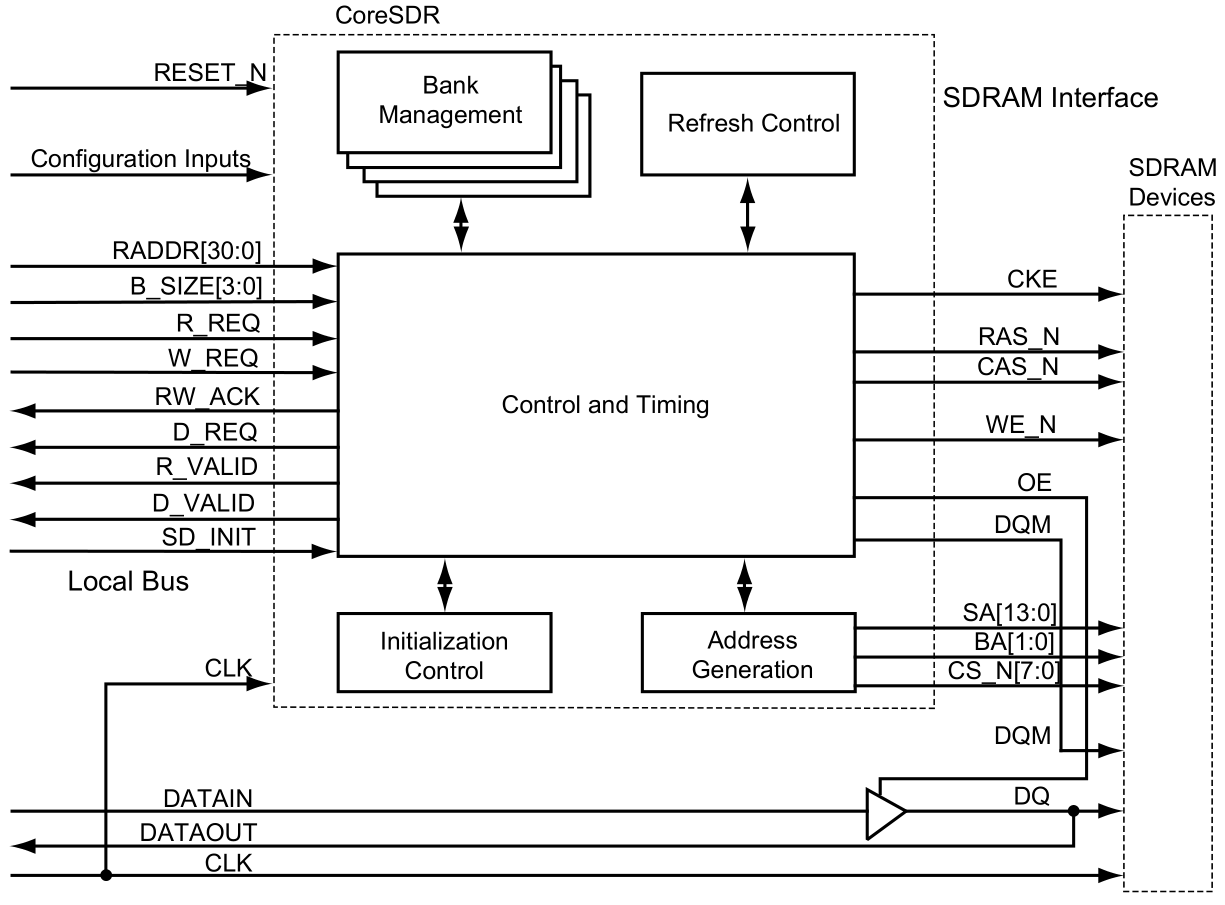
\includegraphics[width=0.7\textwidth]{figures/core_sdr.png}
        \caption{Core SDR architecture diagram overview.}
        \label{fig:core_sdr}
    \end{center}
\end{figure}

\paragraph{Embedded Memories} \mbox{}\\

In order to store the code and data, the SoC solution includes two different types of memories: embedded Non-Volatile Memory (eNVM), using the flash technology; and the embedded Static RAM (eSRAM). For the payload design, the eNVM is dedicated for code storage, constants and runtime variables, which provides to the system all required functions during execution and reboots. Also, since the eNVM is a flash memory, the radiation effects are reduced due to its intrinsic resilience. However, considering that the experiment memories (SDRAM) could generate many bytes of error, in case of block failures, the eSRAM is used to store these logs. This approach guarantee that the system tasks will be properly executed without memory issues due to capacity, since the potentially dangerous growth capable data is stored in a different device. In this scenario, the worst case is achieving the eSRAM memory capacity and overwriting the older results. Then, in order to avoid this problem, a system behavior change is triggered when determine memory usage levels are achieved.

The eNVM has a capacity of 256kBytes that provides a secure size for all the system applications and runtime variables without limitation issues. Moreover, the eSRAM two modules with 32kBytes each when SECDED-ON and 40kBytes each when SECDED-OFF. The single error correction, double error detection (SECDED), a extension of the Hamming code, is a technique to improve the data storage reliability, in this case on the eSRAM, which is less resilient to the radiation effects. Since this algorithm is a built-in feature of the SoC FPGA and the capacity is handled in software, the eSRAM is used with the SECDED enabled. The \autoref{fig:esram} describe the eSRAM scheme in both cases. Then, using this approach, it is possible to avoid potential problems with the system memories, allowing the payload to properly evaluate the radiation effects on the target devices, the SDRAMs. 

\begin{figure}[!ht]
    \begin{center}
        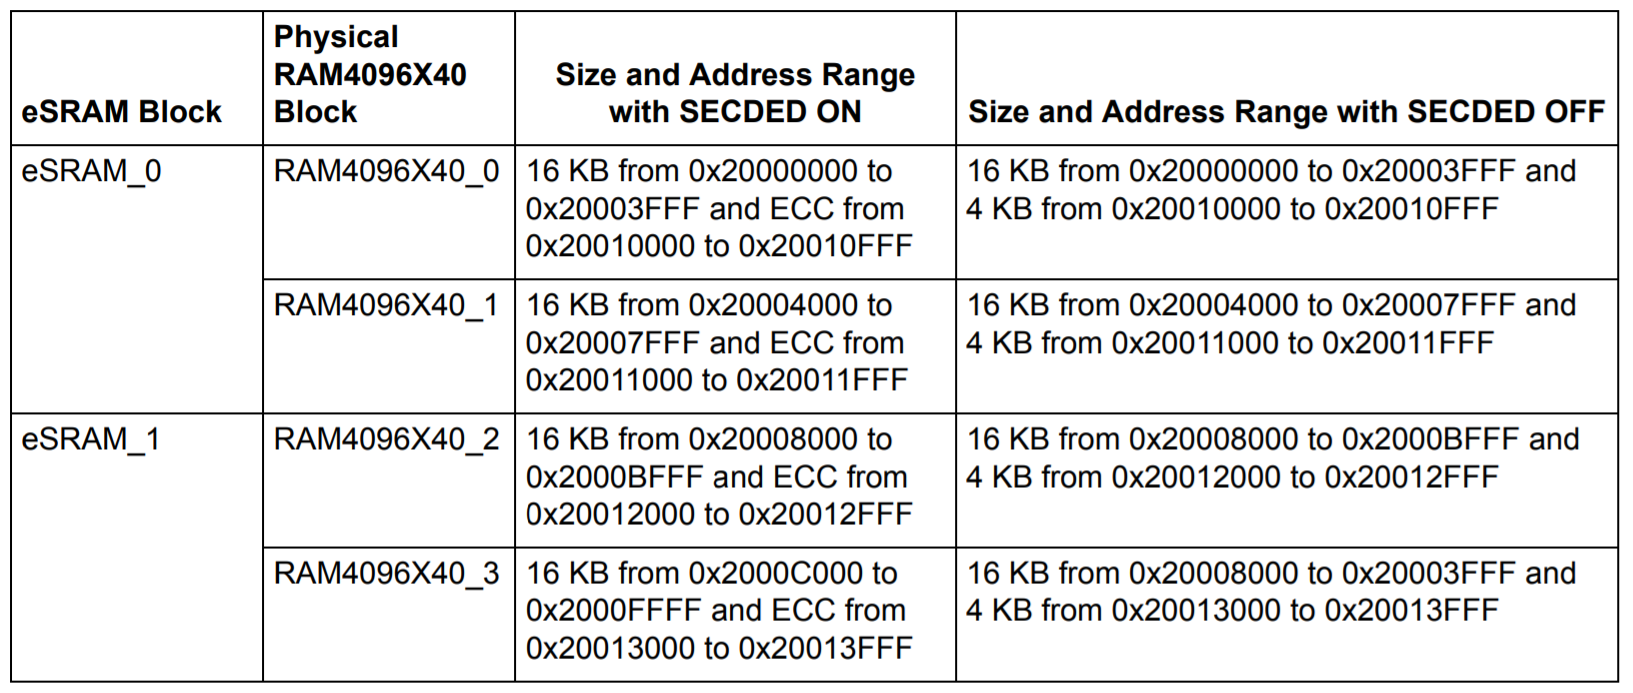
\includegraphics[width=0.7\textwidth]{figures/esram.png}
        \caption{eSRAM memory scheme.}
        \label{fig:esram}
    \end{center}
\end{figure}

\paragraph{Serial Interfaces and IO Ports} \mbox{}\\

The Microsemi FPGA SoC solution provides several peripherals in the MSS subsystem. For this payload, it is used different serial communication protocols (SPI, I2C, CAN and UART) and GPIOs to provide flexibility and redundancy. The SPI protocol, as slave, is used exclusively for communication with the GOLDS-UFSC OBDH. In this interface is used the FloripaSat Protocol (FSP), in order to attend the OBDH requirements and increase the communication reliability. Also, as redundant channels, the I2C (as slave) and CAN could be used for the same interface. This design allows compatibility with further missions of the FloripaSat core, since the payload could be used as a health monitor for radiation damage. Moreover, a UART interface is provided for system logging, which ease the development and debug processes, and a JTAG for the FPGA programming. Also, 20 GPIOs are available for parallel protocols, hardware tests or debugging, 6 IOs for the latch-up monitors and two pins for the FPGA live probes, used for system monitoring during debug. 

These interfaces are available in different connectors, models and locations depending on priority and utilization: SPI, I2C and 4 GPIOs on the contact connector (interface with the OBDH); CAN, JTAG and 14 GPIOs on dedicated connectors; UART, JTAG, live probes and 2 GPIOs on dedicated connectors only available in the engineering model due to space constraints; and the 6 IOs, directly connected to the latch-up connectors. 

\paragraph{Watchdog Timer, Interruptions and Timers} \mbox{}\\

The internal watchdog timer provide a failure recovery feature for the payload system, without the necessity of an external device. This mechanism protects the payload  against software errors by resetting the device and restoring the system execution from boot. Moreover, the payload uses the available timers to synchronize the peripherals execution and trigger system actions, alongside the interruption handler that manages these events.  


%================================================================================

\subsection{Firmware Architecture}

The CubeSat standard, although restrictive concerning definitions of external mechanical and electrical interfaces, integration guidelines and materials utilization, it does not restrain the implementation of the internal subsystems. Regarding the firmware architecture a considerable freedom allows the developers to propose their own standards using approaches and patterns from different application niches. For instance, companies tend to introduce a proprietary architecture in their platforms, creating a tailored environment of modules and development tools \cite{gomspace} \cite{isis} \cite{endurosat}. Moreover, since the CubeSat missions have a substantial contribution from the academic environment, a wide range of techniques and models are employed intending to attend the application requirements and explore novel strategies \cite{polysat} \cite{floripasat}. 

However, these projects share principles and patterns inherent to critical applications, and more specifically, space niche that imply focusing on the same aspects: reliability, environment hardness, redundancy and predictability. Then, regarding the software development, using these concerns to design failure-aware systems generally lead to sophisticated and robust architectures, which increase the mission success probability. Considering the scope of this project, the following sections detail the aspects that guided the payload firmware development, describe the behavioral operation of each module and include the subsystems design.

%--------------------------------------------------------------------------------

\subsubsection{Design Guidelines}

\paragraph{Failure Protection Strategies} \mbox{}\\

The payload firmware is designed to decrease failures due to system malfunctions and environmental conditions. Some of these strategies are periodic system resets, watchdog timer, hardware check routines, default parameter values and error correction algorithms in the system memories and communication interfaces. For instance, the embedded SRAM memories, designated to store the experiment results, use the Single Error Correction, Double Error Detection (SECDED), a extension of the Hamming code. Also, in the communication with the GOLDS-UFSC OBDH, a Cyclic Redundancy Check (CRC) algorithm, an error-detecting code used to detect accidental changes to raw data, is applied inside the interface protocol. 

Moreover, the payload firmware in based on an operating system targeted to the embedded systems, which improves the overall reliability since the platform has inheritance of several projects in different applications, including in the space sector. Then, using this framework to develop the payload firmware, the system failures are mitigated and the architecture more qualified to the application.


\paragraph{Internal and External Synchronization} \mbox{}\\

The system synchronization within internal constraints and with external devices is a challenge since the payload is intended to operate controlled by the OBDH and, meanwhile, perform several functions within certain time and priority limitations. Then, using the operating system framework, this requirement is accomplished using queues, tasks and semaphores and interruption handlers, which provide tools to accommodate the different constraints in a deterministic fashion. In summary, each task has an execution rate, priority and optional parameters (semaphores, initial delays and group events) that are predictably handled by the framework scheduler. Besides this execution scheme, data should be transferred between these task without the necessity to be immediately handled, which is the fundamental strategy of the data synchronization. Also, since the system operation is controlled by the OBDH (slave mode), it is necessary a interruption handler for communications, which is non-deterministic and could cause issues. Then, to avoid this problem, a binary semaphore is used to create a link between the interruption occurrence and a handler task, which transforms the operation deterministic in terms of execution alongside rest of the system tasks. 

Moreover, the communication with the OBDH has synchronization strategies due to the FloripaSat Protocol (FSP), which defines a communication standard between both modules. This protocol uses handshake operations, acknowledge responses and set a command list, besides error-detecting routines to ensure correct communication. 
These herein strategies and features are detailed in depth throughout the following sections, reveling the actual architecture, operation mechanisms and consequences.


\paragraph{Abstraction Layers} \mbox{}\\

The firmware structure is based on abstraction layers, which create a separation between layers and allow a development oriented to the application itself instead of the hardware details in that feature. Also, this strategy increase the firmware readability, flexibility, organization and maintenance, due to the implementation independence from distant layers and abstraction of unnecessary information. The \autoref{fig:abstraction_layers} presents this layers and their hierarchy. At the bottom, it is represented the lowest level, the SoC implementation, then the first abstractions, called hardware abstraction layers due to handling with specific operation related with the processor and peripherals. At the upper levels, there are the application layers that use a high-level description approach for the implementation of the payload system functionalities and operations.  

\begin{figure}[!ht]
    \begin{center}
        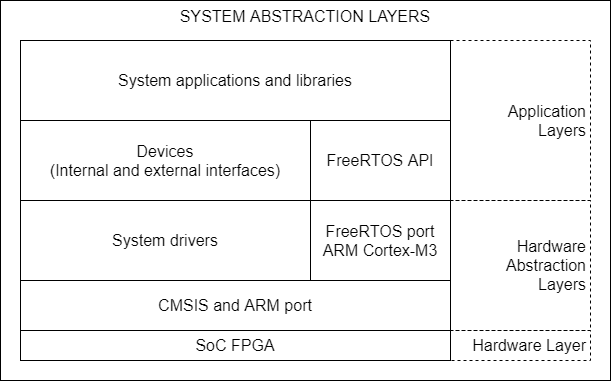
\includegraphics[width=0.7\textwidth]{figures/abstraction_layers.png}
        \caption{System abstraction layers diagram.}
        \label{fig:abstraction_layers}
    \end{center}
\end{figure}


%--------------------------------------------------------------------------------

\subsubsection{Design Overview}

The firmware architecture, as herein described, use an embedded operating system that is widely used in commercial products. The FreeRTOS is a real-time operating system (RTOS) for microcontrollers and small microprocessors with proven robustness, tiny footprint, and wide device support. Then, in order to use a similar architecture as the GOLDS-UFSC OBDH, share libraries and ease the development process, the FreeRTOS was the most feasible platform for this project, besides the official port for the Microsemi SmartFusion2 SoC FPGA devices. This firmware development approach lead to the conception of functionalities translated into operating system tasks and synchronization schemes in queues and semaphores. In summary, the firmware is designed using the operating system features and structure. 

Regarding the system functionality, the \autoref{fig:system_flow} describes a simplified execution diagram, presenting the main experiment functions and their sequence. The housekeeping and system functions are omitted to evidence the major payload purpose, the experiment execution itself. After power-on and internal setup, the payload receives a command from the OBDH, prepares the experiment parameters and enables the experiment execution. Then, this data is stored in the embedded SRAM for later retrieve when a OBDH data request occurs. This loop summarizes the experiment application and the payload purpose, evaluate the SDRAM memories in the harsh environment.

\begin{figure}[!ht]
    \begin{center}
        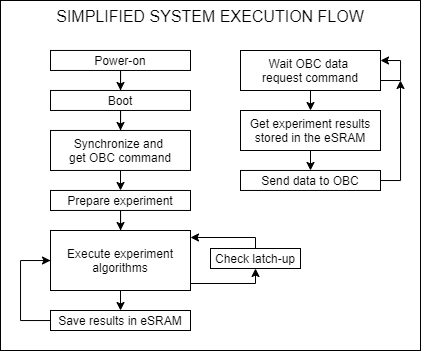
\includegraphics[width=0.55\textwidth]{figures/system_flow.png}
        \caption{Simplified system execution flow diagram.}
        \label{fig:system_flow}
    \end{center}
\end{figure}

These functionalities, as herein noted, are translated in tasks, queues, semaphores and interrupt handlers, which are represented in the \autoref{fig:system_architecture}. Also, some parameters are presented (priority, rate, periodicity and depth) that are detailed and justified in the following topics.

\begin{figure}[!ht]
    \begin{center}
        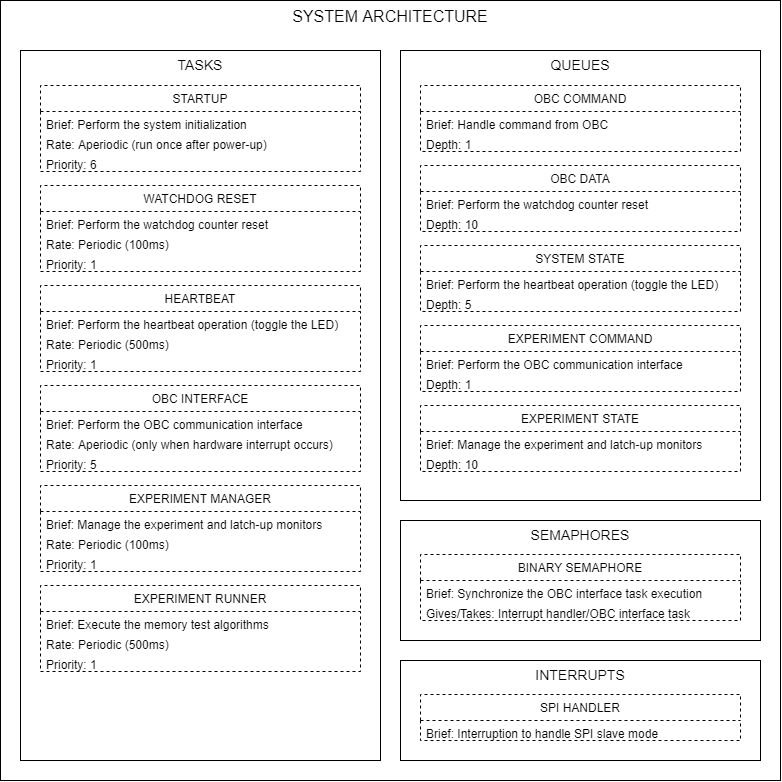
\includegraphics[width=0.8\textwidth]{figures/system_architecture.png}
        \caption{System architecture diagram.}
        \label{fig:system_architecture}
    \end{center}
\end{figure}

\paragraph{Experiment Routines} \mbox{}\\

The experiment is executed through two dependent and periodic tasks: "experiment manager task" and "experiment runner task". The first is responsible to handle the commands received through the communication, constantly check the latch-up monitors, and coordinate the system queues. The second task coordinate the experiment execution and save the generated experiment data results. Concerning the execution flow, the manager task has a higher priority than the runner one, thereby executing despite the experiment cycle accomplished the end. This design would lead to issues if a synchronization mechanism did not coordinate the execution of one task accordingly to the other. Then, in order to fulfill this need a queue system was designed to trigger some states that are executed in key moments, for instance: reading the memory to restore the experiment results, changing the execution configuration parameters, and many other functionalities. 

There are two queues directly used in the experiment routine and three indirectly, which transfer data, configuration parameters and status. The two direct queues are used for receiving the configuration from the manager to the runner task, and sending the position and size of the experiment data stored in the dedicated memory sector to the manager task. The other queues are used by the manager and communication tasks for inputting the commands from the OBC, and outputting the data and status information to the OBC.  

The \autoref{fig:experiment_architecture} summarizes the experiment execution flow, presenting from the communication with OBC to the execution of the memory test algorithms. It starts with the command received from OBC, process the execution parameters, run the test algorithms, store data in the dedicated memory, send data status for further retrieving, read this data, and finishes sending it to the OBC. This sequence is a simplified overview and support the visualization of the routine, but it should be analysed as two tasks not necessarily contiguous in time and using queues to trigger sequential events.  

\begin{figure}[!ht]
    \begin{center}
        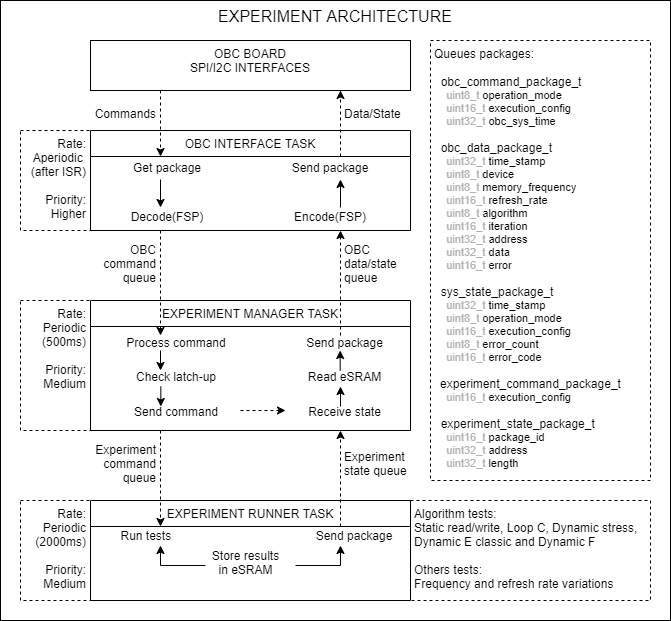
\includegraphics[width=0.8\textwidth]{figures/experiment_architecture.png}
        \caption{Experiment architecture diagram.}
        \label{fig:experiment_architecture}
    \end{center}
\end{figure}

\paragraph{Housekeeping Routines} \mbox{}\\

The housekeeping routines are responsible to initialize and maintain the system properly configured and operational. There is an aperiodic task referred to as "startup" that performs the system boot once after power up, in other words, the initialization of all peripherals, interfaces, and devices. Also, there is a dedicated periodic task that ensures constant notification of properly operation for the watchdog timer and another one with the lowest priority for other periodic non essential functions (e.g., blink LED).

\paragraph{Communication Routines} \mbox{}\\

The communication routines are handled using an aperiodic task and interruptions (one for each physical protocol). The task execution trigger is associated with the interruption since the payload is a slave in the communication from the perspective of the OBC. Then, to ensure that the communication is correctly attended, the task has the highest priority. This strategy is adopted to accomplish both requirements, attend communication requests with low latency and use the payload firmware formal application structure (i.e., the operating system tasks). Also, this method prevents conflicts between the scheduler and manually configured interruptions, and allows the use of the operating system features safely. The \autoref{fig:interrupt_freertos} presents the scheme adopted to receive and process the communication interactions. Also, the \autoref{fig:experiment_architecture} describes the interface of the communication task with the experiments routines using queues for synchronization.

\begin{figure}[!ht]
    \begin{center}
        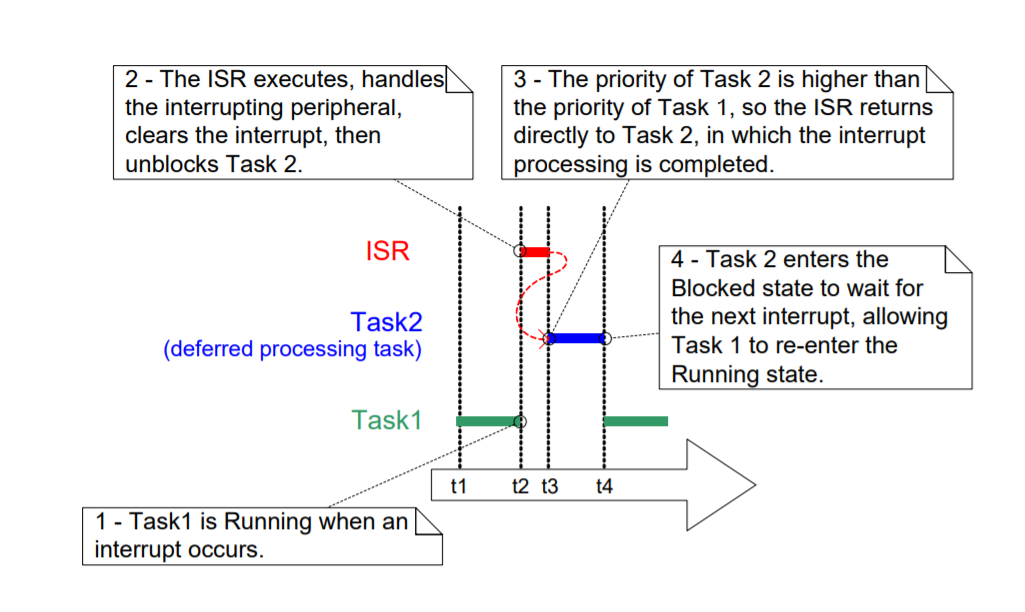
\includegraphics[width=0.75\textwidth]{figures/interrupt_freertos.png}
        \caption{Communication interrupt and task architecture diagram.}
        \label{fig:interrupt_freertos}
    \end{center}
\end{figure}

\paragraph{Debug and Logging Routines} \mbox{}\\

In order to perform debug sections and execute integration tests, there is a logging system to provide useful feedback during the development. The routines use a serial interface (UART) to output relevant steps and notify critical failures, which are easily read through a serial monitor (i.g., PuTTY or equivalent). These logs are inserted in key positions, using status flags to select between appropriate messages.

%--------------------------------------------------------------------------------

\subsubsection{Memory Fault Detection Algorithms}

There are two subcategories of memory detection algorithms: static, more generic and global error detection, and dynamic, which try to catch specific errors when they occurs (usually are model and technology dependent). Due to the general purpose characteristic and simplicity of the static algorithms, this work implemented two static algorithms. The first is a simple verification that performs write operations in all the memories address space with a specific value and later, after some adjustable period, it is read and compared with that value. In case of faults, the algorithm reports relevant information about the execution. The second algorithm follows a similar approach, but divide the memory in different sized portions and performs a correction attempt to ensure that the fault was a radiation functional problem and not a communication error. Despite similar, the methods have different sensibility for certain faults and are better applied in distinct scenarios. For example, the first is more prone to single event upsets than the second or the second is more reliable at the expense of execution speed.


%================================================================================

\subsection{Hardware Architecture}

The payload hardware consists of a 6-layer PCB, using the GOLDS-UFSC OBDH DaughterBoard standard and following simplified space application design guidelines. In order to enumerate this patterns and constraints, the following section describes the applied techniques and particularities of the payload design. Then, each developed modules receives a brief architectural and functional description. Moreover, the tests results are analysed to evaluate the requirements accomplishment and developed functionalities.        


%--------------------------------------------------------------------------------

\subsubsection{Preliminary Design Analysis} \label{subsec:hard_design_analysis}

\paragraph{Layer Stackup Planning} \mbox{}\\

The payload layers scheme were specified to attend the rules described herein and to increase the feasibility of production, which uses convenient dimensions for the target manufacturer. Since the engineering model do not require space qualified boards, this scheme allowed to reduce the costs and time during this process. The \autoref{fig:stackup} describe the payload stackup, including: layers, dimensions and characteristics. In order to avoid tracks in the external layers, the strategy was to use the middle ones for routing, permitting the shield properties of these external layers and suitable power planes in the internal ones. Moreover, to reduce crosstalk between the signal layers, they are orthogonal concerning the routing preferential directions. Also, despite the external layers assigned for ground reference, some parts are used to handle the external supply voltages to prevent splitting the power plane, which lead to efficiency reduction as low impedance reference and increase the return paths. In summary, to correctly employ this stackup, the internal layers must have the lowest impedance (short return paths) and the external providing electromagnetic interference shielding.  

\begin{figure}[!ht]
    \begin{center}
        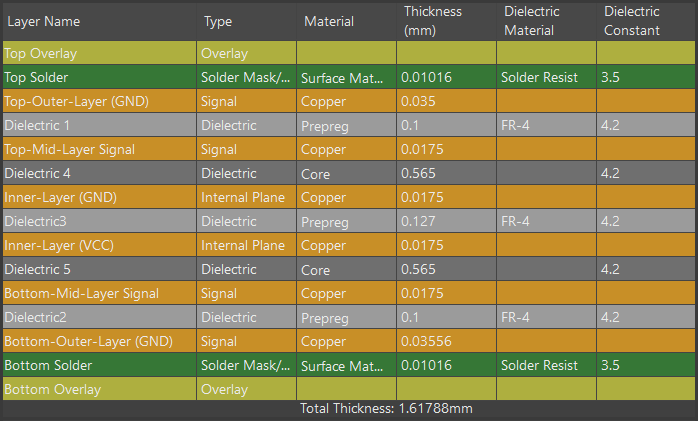
\includegraphics[width=0.6\textwidth]{figures/stackup.png}
        \caption{Stackup planning.}
        \label{fig:stackup}
    \end{center}
\end{figure}

\paragraph{Placement Planning} \mbox{}\\

The components placement were defined using the external connectors accessibility, considering the position in relation to the motherboard (the GOLDS-UFSC OBDH), and internal requirements. However, the positioning of the FPGA device and memory chips were the major factor considered, since the most critical routing is between these components. Also, to ease the layout development process, the memories were placed symmetrically placed in relation to the FPGA and uniformly distributed in the board. The \autoref{fig:fpga_pinout} present the FPGA pin assignment to attend these requirements. It is important to note that the DDRIO and MSIOD banks were not used due to the maximum voltage levels allowed, 2.5 Volts. This assignment scheme provide three groups of signals in different directions, which ease the BGA fanout and tracks escape routes: memory control and address signals; memory data signals; and general purpose inputs and outputs.

\begin{figure}[!ht]
    \begin{center}
        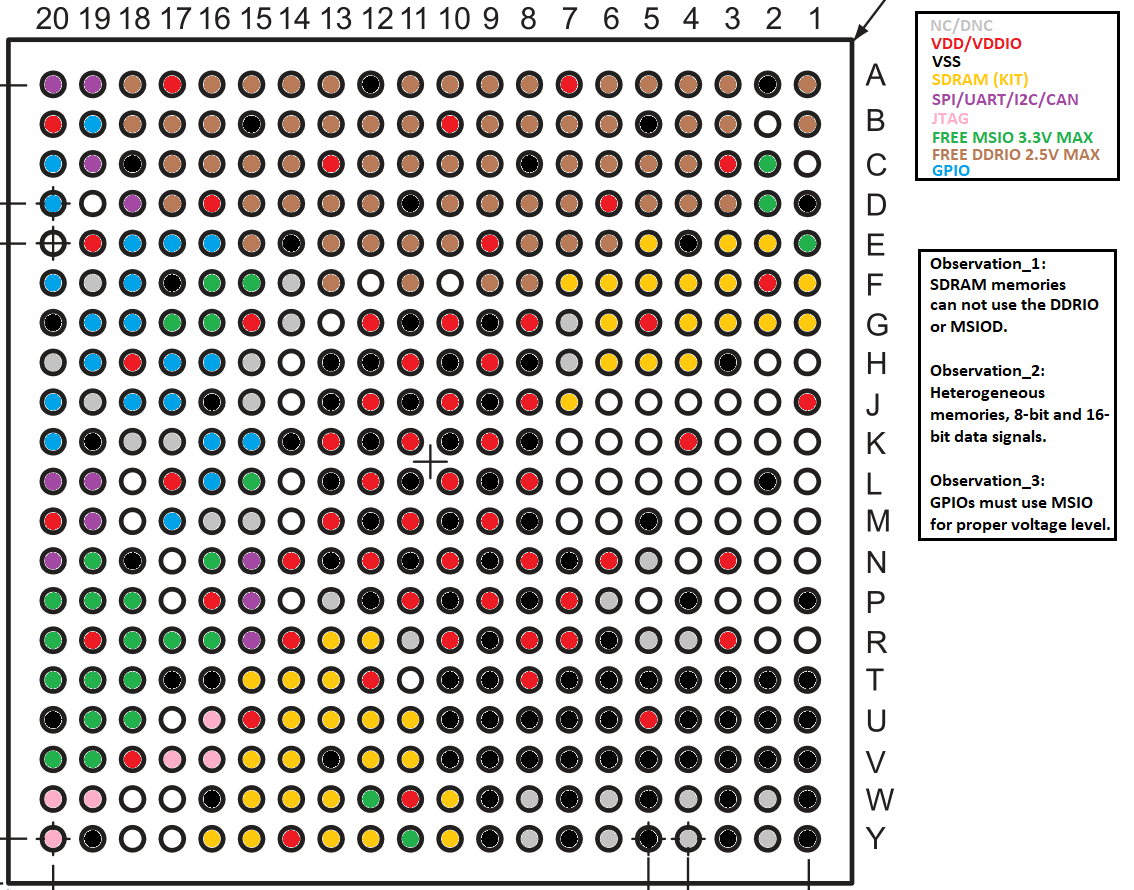
\includegraphics[width=0.6\textwidth]{figures/FPGA_pinout_prototype.png}
        \caption{FPGA pinout usage.}
        \label{fig:fpga_pinout}
    \end{center}
\end{figure}

\paragraph{High-Speed Design Planning} \mbox{}\\

The board component interfaces are in the edge of being considered as high-speed signals due to the SDRAM memories. Then, even if a more complex approach is not required for this work, some measures were considered in the payload design to avoid issues and bad performance. The most important strategy is the properly grounding and power planes for return signals, which were herein described in the stackup planning topic. Also, an orthogonal and similar length routing strategies were adopted to avoid crosstalking and latency issues in the memory signals. The memories are placed symmetrically to provide an easier and organized pattern for routing. 

The \autoref{fig:mem_addr_sig_top} presents the signal layer used for tracing from the FPGA to the memory chips. The highlighted tracks are the address signals that are routed together to mitigate the length mismatch. The other signals are grouped together depending on their purpose, control or data signals.

\begin{figure}[!ht]
    \begin{center}
        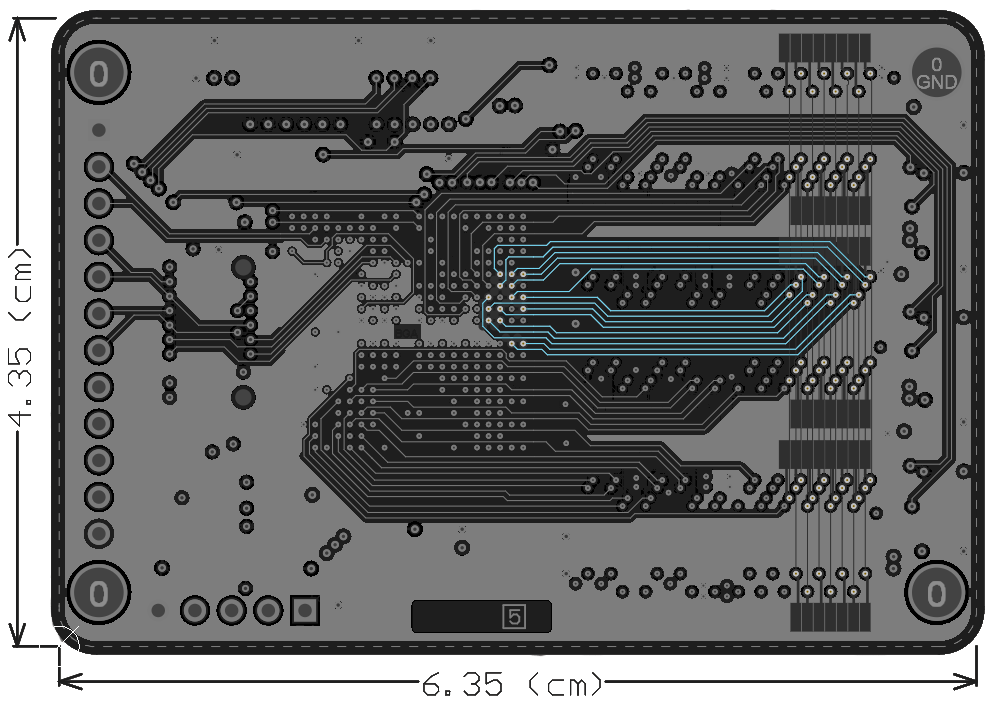
\includegraphics[width=0.55\textwidth]{figures/mem_addr_signals.png}
        \caption{Top Mid-layer routing with focus on the memory address signals.}
        \label{fig:mem_addr_sig_top}
    \end{center}
\end{figure}

The \autoref{fig:mem_addr_sig_bot} shows a similar overview of the same address signals, but presenting them in the other signal layer. The tracks are traced in the shortest routes as feasible and provide the required parallel connections, since the three memories share the same controller pins interface. 

\begin{figure}[!ht]
    \begin{center}
        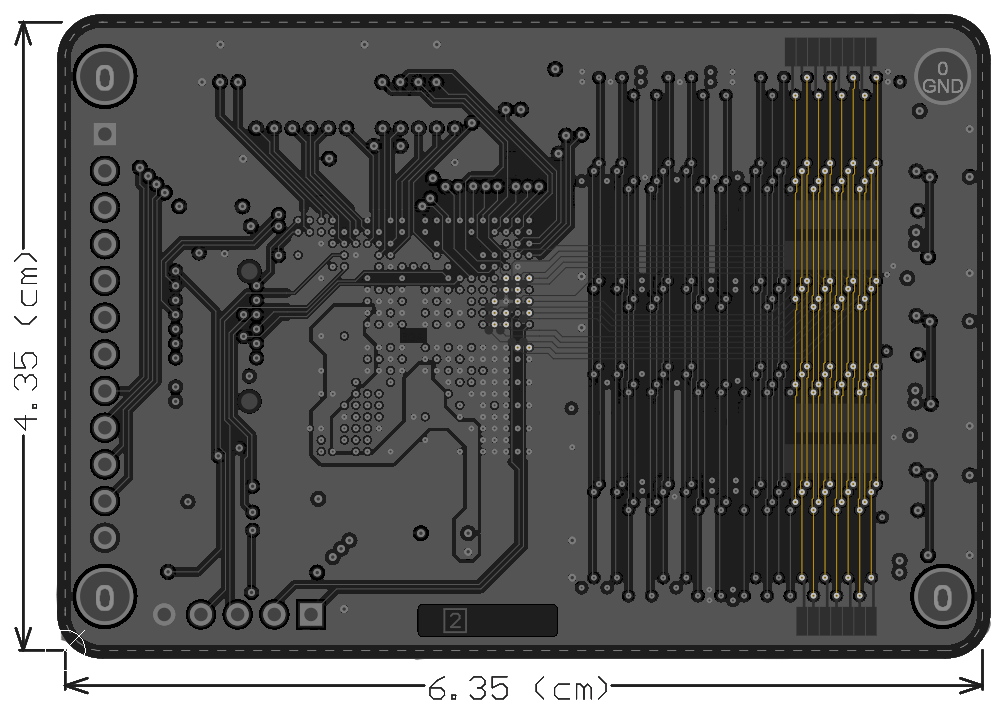
\includegraphics[width=0.55\textwidth]{figures/mem_addr_signals_2.png}
        \caption{Bottom Mid-layer routing with focus on the memory address signals.}
        \label{fig:mem_addr_sig_bot}
    \end{center}
\end{figure}



%--------------------------------------------------------------------------------

\subsubsection{Design Overview}

In summary, the payload hardware essentially consists of a controller, to manage communication and memories, and the SDRAM devices under experiment. However, some auxiliary components and modules are necessary to handle other tasks and fulfill the requirements, including: power converter, to supply the correct FPGA voltage; latch-up monitors, to prevent catastrophic system failures and provide additional data for the experiment; debug support for power supply, logging and programming; additional communication modules and connectors; and the motherboard interface connector. The \autoref{fig:hardware_architecture} presents the payload subsystems, internal connections and external interfaces, besides an internal overview of the SoC FPGA device implemented architecture.

\begin{figure}[!ht]
    \begin{center}
        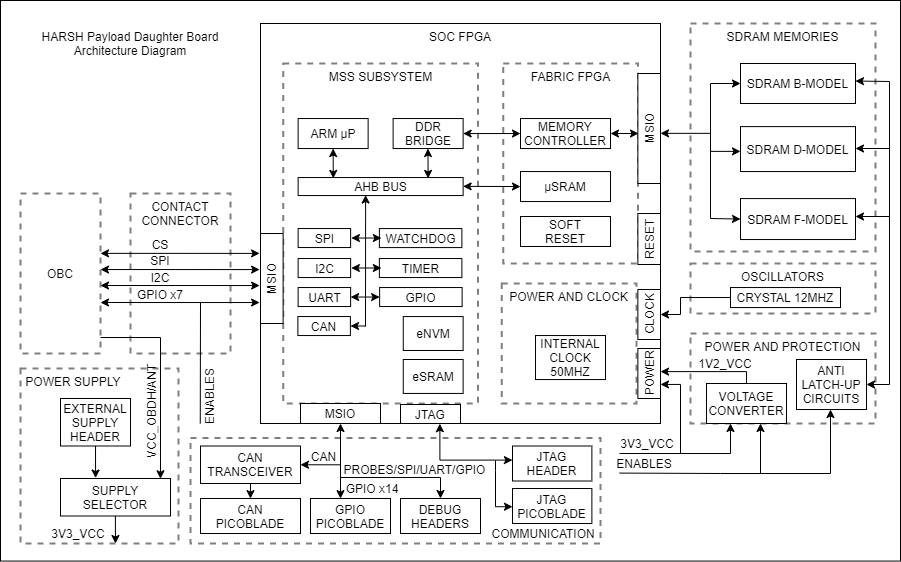
\includegraphics[width=\textwidth]{figures/hardware_architecture.png}
        \caption{Hardware architecture overview.}
        \label{fig:hardware_architecture}
    \end{center}
\end{figure}


In addition to the summarized power supply architecture herein presented, the \autoref{fig:power_architecture} presents in more details the power line names, voltages, and currents, besides their relation with the latch-up monitors.

\begin{figure}[!ht]
    \begin{center}
        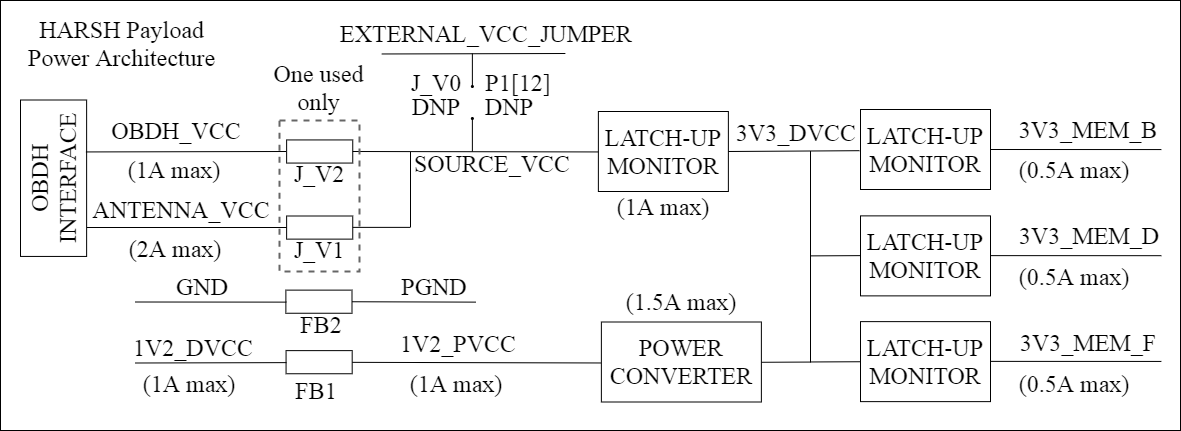
\includegraphics[width=0.8\textwidth]{figures/power_architecture.png}
        \caption{Power architecture overview.}
        \label{fig:power_architecture}
    \end{center}
\end{figure}

The \autoref{fig:harsh_pcb_preview_3d} presents a rendered view of the board top and bottom layers with indications where each module is situated, and the \autoref{fig:harsh_pcb_preview_real} shows the manufactured board. The following topics describe these subsystems functionality and characteristics. Also, in the schematics section of the \autoref{sec:annex_schematics}, the schematics and layers prints are presented.

\begin{figure}[!ht]
    \begin{center}
        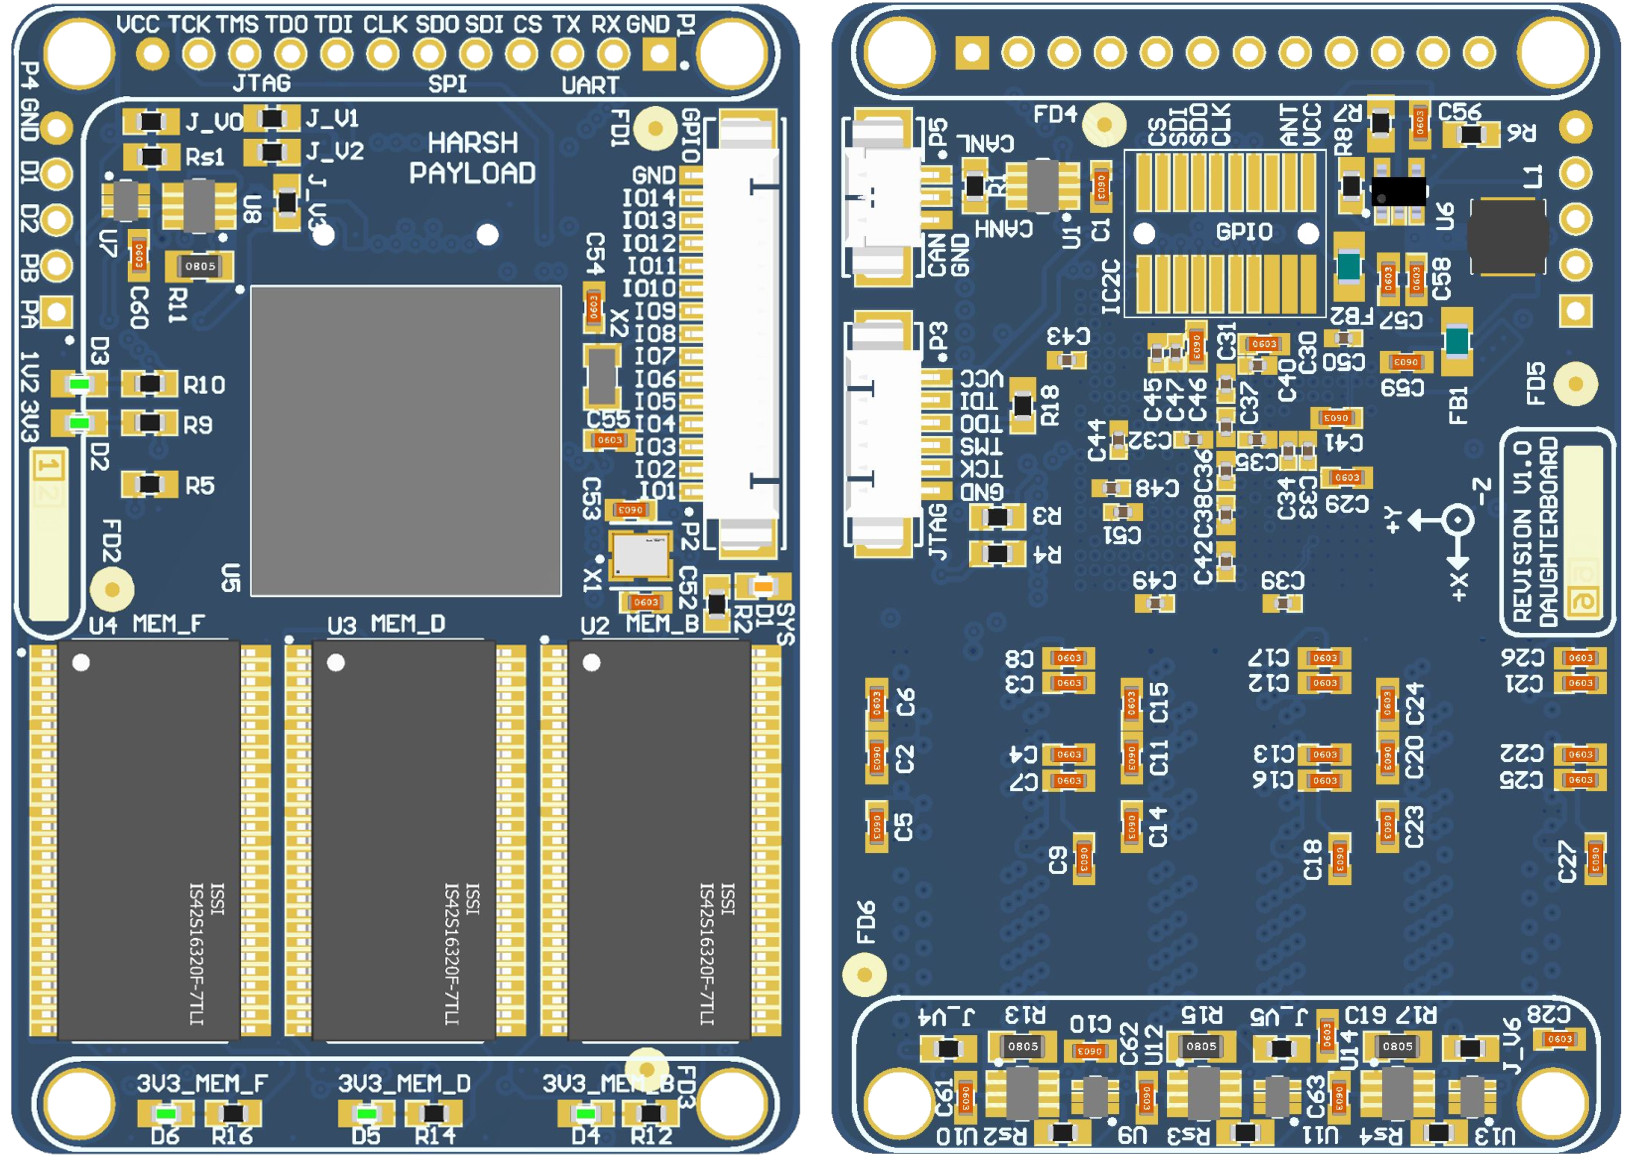
\includegraphics[width=0.9\textwidth]{figures/harsh_pcb_preview_3d.jpeg}
        \caption{PCB 3D rendering overview.}
        \label{fig:harsh_pcb_preview_3d}
    \end{center}
\end{figure}

\begin{figure}[!ht]
    \begin{center}
        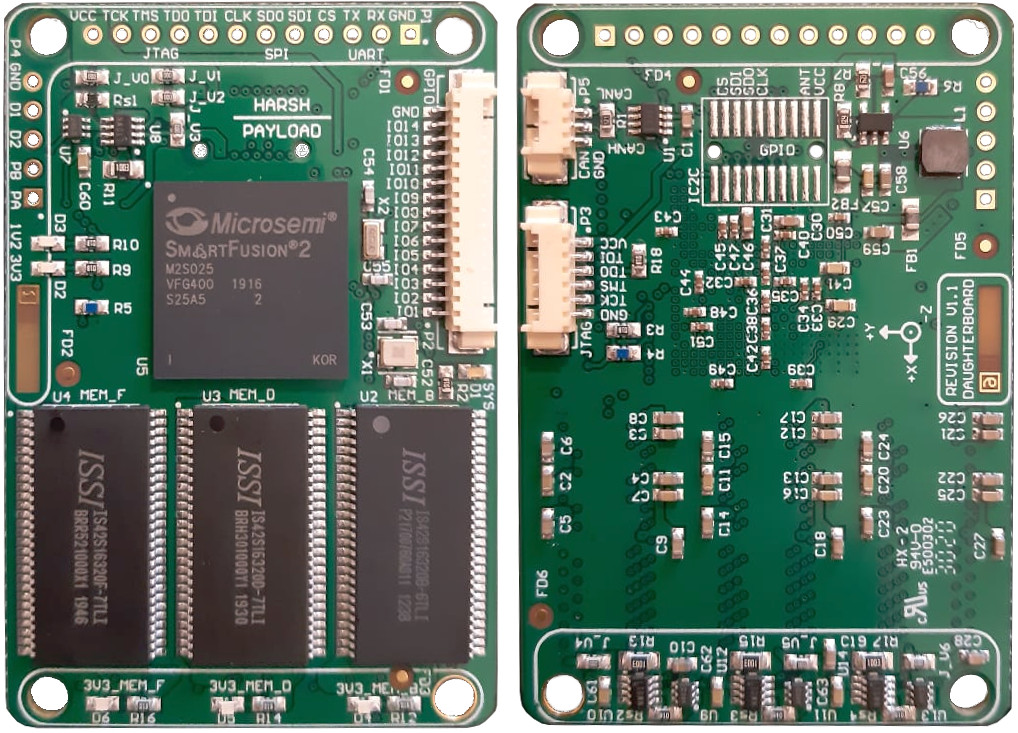
\includegraphics[width=0.9\textwidth]{figures/harsh_pcb_preview_real.jpeg}
        \caption{PCB manufactured overview.}
        \label{fig:harsh_pcb_preview_real}
    \end{center}
\end{figure}

\paragraph{SoC FPGA Module} \mbox{}\\

The FPGA device is a Ball Grid Array (BGA) component that require a fanout implementation and escape routes for the internal pins. The adopted strategy for this work is the dog-bone pattern, which is a widespread technique and attend the project necessities. The \autoref{fig:fpga_fanout_caps} present the implemented pattern and escape routes and decoupling capacitor placement, both using a top view of the board. Since several FPGA pins are not used and the board placement favors the routing, this implementation only required two signal layers and two power planes, which attend the payload specification.

\begin{figure}[!ht]
    \begin{center}
        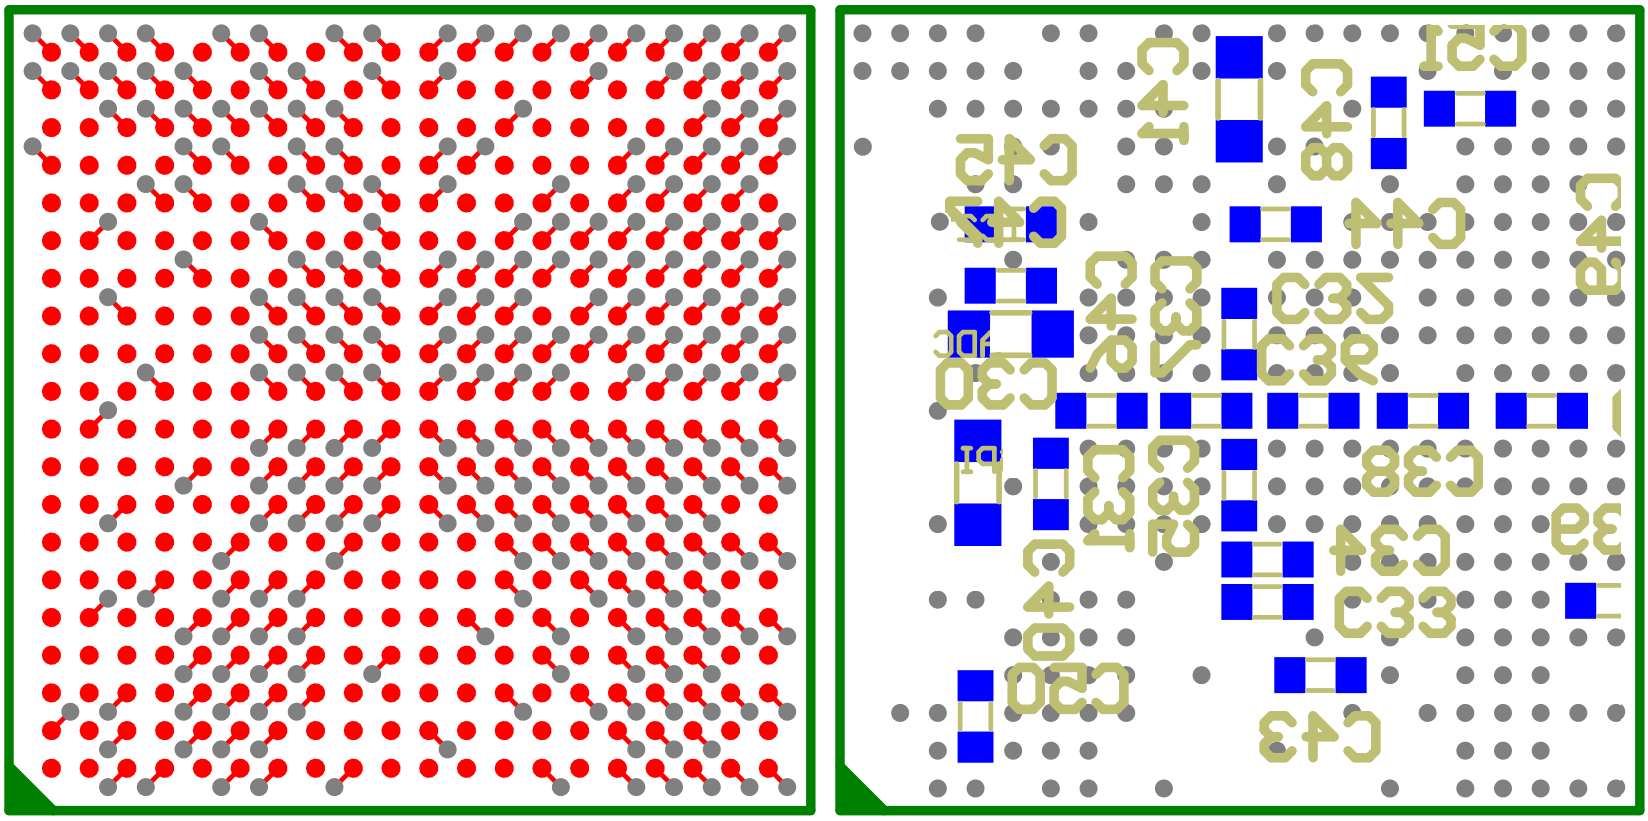
\includegraphics[width=0.8\textwidth]{figures/fpga_fanout_caps.png}
        \caption{FPGA fanout dog-bone pattern and decoupling capacitors implementation.}
        \label{fig:fpga_fanout_caps}
    \end{center}
\end{figure}

\paragraph{Memories Module} \mbox{}\\

The memories module is composed of the three experiment memory chips: IS42S16320B, IS42S16320D, and IS42S16320F. These devices are 512Mb (or 64MB) Single Data Rate (SDR) SDRAMs operating at 3.3V and up to 143MHz in a 54-pin TSOP-II packaging. A SDR device means that it can only read/write one time in a clock cycle, differing from its successors Double-Data Rate (DDR) memories that perform two operations per cycle. The selected parts configuration has a 16-bit data width and the industrial grade qualification.

The target operation frequency is 100MHz using the other parameters in the nominal indications, except for the refresh frequency (8K cycles every 64ms) that might be changed during some experiment tests. The electrical topology is a parallel connection that shares the same controller interface. This strategy was adopted since it saves the usage of several FPGA pins and the used configuration is the same. 

During the board design, as presented in the Figures \ref{fig:harsh_pcb_preview_3d} and \ref{fig:harsh_pcb_preview_real}, the placement was selected to avoid any component unrelated to the memories be located on their opposite side. Also, this measure ensures that the decoupling capacitors are as close as possible of their power pins. Regarding the routing, the strategies employed were described in the \autoref{subsec:hard_design_analysis}.

\paragraph{Communications and Debug Interfaces} \mbox{}\\

The payload uses several communication interfaces distributed in different connectors according to the requirements or usage. There are six available interfaces for different purposes: SPI, JTAG, UART, I2C, GPIOs, and CAN. The SPI, JTAG, and UART are the main used communication protocols and the rest were added for redundancy or additional non critical features. In the same scheme, there are six different connectors that share some interfaces: 3 picoblades, 2 debug headers, and 1 contact connector. The debug headers are not used in the flight configuration due to size limitation.

The picoblades are separately utilized for a CAN channel, a JTAG interface, and the application GPIOs. The debug headers provide an easier access for the UART logger, the application SPI, a JTAG interface, debug GPIOs, and a external power supply input for debug. The contact connector is the main interface with the OBC, which provides the application SPI, an I2C for redundant communication, OBC power inputs, and the control GPIOs.

This approach was adopted to improve the design flexibility and allow the adaptation of the payload for different scenarios. For instance, it is planned to perform ground experiments before the payload launch and also the possibility of utilization in different satellite missions.

\paragraph{Power Module} \mbox{}\\

The power subsystem is composed of a DC converter and a simple noise filtering network. In the payload specification is stipulated that a 3.3V power line is reserved for supplying the board, which should ensure current limitation in case of a latch-up. This requirement is accomplished using a anti latch-up circuitry and through the power converter protection as a redundancy.

In order to supply the 1.2V for the FPGA chip, there is a Direct Current (DC) switching power converter (TLV62565DBVR). This step-down converter operates with high efficiency (above 85\%), supplying up to 1.5A with overcurrent and thermal protections. The selected part is a 5-Pin SOT-23 chip and features an enable input. 

The noise filtering network is the combination of four passive components: two ferrite inductors and two ceramic capacitors. This circuit filters the high frequency noises generated by the switching converter and received from the OBC. Then, there are 1.2V power lines and power grounds before and after the filter, which allows better signal performance for the rest of the circuits. 


\paragraph{Latch-up Monitors} \mbox{}\\

The latch-up circuitry consists of four monitors: one for the entire board and three for individually controlling the experiment memories. The circuit is based on the LTC4361ITS8-1 device that provides the required overcurrent protection through the management of a MOSFET transistor (SI1416EDH-T1-GE3). The monitor uses a SOT-8 package and the transistor chip a SOT-363-6 package, which offers a compact and efficient solution. This system is completely independent for opening the circuit in case of non nominal condition, but dependent for closing again. The memory monitors are controlled by the SoC FPGA in case of an event and the general monitor is only controlled by the OBC, since the payload is completely turned off during this condition. The system also provides a status pin that is used for detecting these events. 


%================================================================================

%\\6.4 Development API for OBDH

\clearpage